%% $RCSfile: proj_report_outline.tex,v $
%% $Revision: 1.3 $
%% $Date: 2016/06/10 03:41:54 $
%% $Author: kevin $

\documentclass[11pt
              , a4paper
              , twoside
              , openright
              ]{report}


\usepackage{float} % lets you have non-floating floats

\usepackage{url} % for typesetting urls

\usepackage[final]{pdfpages}

%
%  We don't want figures to float so we define
%
\newfloat{fig}{thp}{lof}[chapter]
\floatname{fig}{Figure}

%% These are standard LaTeX definitions for the document
%%                            
\title{aWall: Collaboration Support for Agile Retrospectives}
\author{Simon Glew}

%% This file can be used for creating a wide range of reports
%%  across various Schools
%%
%% Set up some things, mostly for the front page, for your specific document
%
% Current options are:
% [ecs|msor|sms]          Which school you are in.
%                         (msor option retained for reproducing old data)
% [bschonscomp|mcompsci]  Which degree you are doing
%                          You can also specify any other degree by name
%                          (see below)
% [font|image]            Use a font or an image for the VUW logo
%                          The font option will only work on ECS systems
%
\usepackage[image,ecs,mcompsci]{vuwproject}

% You should specifiy your supervisor here with
%     \supervisor{Firstname Lastname}
% use \supervisors if there is more than one supervisor

\supervisor{Dr. Craig Anslow}
\otherdegree{Bachelor of Engineering with Honours}

% Unless you've used the bschonscomp or mcompsci
%  options above use
%   \otherdegree{OTHER DEGREE OR DIPLOMA NAME}
% here to specify degree

% Comment this out if you want the date printed.
\date{}

\begin{document}

% Make the page numbering roman, until after the contents, etc.
\frontmatter

%%%%%%%%%%%%%%%%%%%%%%%%%%%%%%%%%%%%%%%%%%%%%%%%%%%%%%%

%%%%%%%%%%%%%%%%%%%%%%%%%%%%%%%%%%%%%%%%%%%%%%%%%%%%%%%

\begin{abstract}

This is a problem as it means either product teams have to either be co-located or have to be all parts of agile meetings using a third party meeting tool such as Skype. 
Integrating an agile retrospective method within aWall will allow users to do all agile meetings within one online agile tool.  

\end{abstract}

%%%%%%%%%%%%%%%%%%%%%%%%%%%%%%%%%%%%%%%%%%%%%%%%%%%%%%%

\maketitle

%%%%%%%%%%%%%%%%%%%%%%%%%%%%%%%%%%%%%%%%%%%%%%%%%%%%%%%

\mainmatter

%%%%%%%%%%%%%%%%%%%%%%%%%%%%%%%%%%%%%%%%%%%%%%%%%%%%%%%

% individual chapters included here
\chapter{Introduction}\label{C:intro}
\section{The Problem} 
The problem that this project is to solve is attempting to support agile retrospectives meetings through touch walls and screens, this is going to be done by creating a prototype application that will be used to support them. This project is part of the aWall software project run by Dr. Craig Anslow and Professor Martin Kropp of FHNW in Switzerland. aWall is a digital touch application to manage the different agile processes within a team such like Sprint Planning and Agile Retrospectives.\\
Agile Retrospectives are meetings held within teams once complementing an increment of work. They allow teams to inspect and adapt the different areas that are required within themselves and allow for change and learning within the entire team \cite{AgileRetrospectivesEstherDerby}.

The outcome of this project, is to build a software web system to help facilitate agile retrospective meetings using a large touch screen as an output for the software. Once this software has been built, an evaluation with users will occur to evaluate and improve on the software project. The current aWall project can be found here: \url{https://www.youtube.com/watch?v=fzCnjnpRiTI}

\begin{figure}[ht]
	\centering
	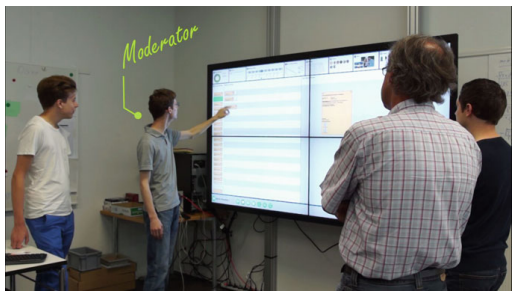
\includegraphics{aWall_introduction}
	\caption{Project aWall - digital agile cardwall being used \cite{xp2017_aWall}}
\end{figure}

\section{Overview of Research Project}
This project will be building off this current prototype but within its own project scope and no integration between the two codebases.

This software prototype is split into three different components:
\begin{itemize}
	\item \textbf{Participant System:} The participant system is used for the participants to interact within the system, it is an application that will allow the participant to vote and make notes about the retrospective and directly interact with what is happening on the screen and within the retrospective. All the interactions from this system get seny and stored within the database housed within the server. This system will be accessed from a secondary device by the user e.g their phone. This system sets up a connection to the server through a socket, allowing for the required transfer of data.
	\item \textbf{Screen System:} The screen system is an application that the moderator of the retrospective interacts with, it allows the moderator to display and manipulate the data passed from the server that the participants have given. This system will be used on the touch screen with a connection to the server through a socket.  
	\item \textbf{Server:} The server houses all the data storage and manipulation for the overall software system. The server also houses the socket system allowing for real-time updates between the participant and screen systems. The server allows the storage of data for futher use in later iterations of the projects lifecycle, e.g. a later agile retrospective. 
\end{itemize}

Within this prototype there will be different versions of agile retrospectives that the different members of the agile team can choose. The different retrospectives that were chosen through doing a background review on the different retrospectives methods that where found. The ones that were chosen either linked up with the other two sections of a retrospective nicely or were found within multiple different sources \cite{AgileRetrospectivesEstherDerby, normanKeith}. The retrospective methods that were chosen are:
\begin{itemize}
	\item The 3W's/Mad, Sad and Glad
	\item Timeline
	\item Brainstorm/Filtering
	\item Short Subjects
\end{itemize}

Each of these retrospective methods will be able to be selected from the screen system within the software application when creating a retrospective session. To accompany each of these retrospective methods, there will also be short sections before and after the main method, it allows for the setting of the scene within the retrospective and to wrap up the retrospective also.

The methods that I have chosen for this are:  \cite{AgileRetrospectivesEstherDerby}
\begin{itemize}
	\item \textbf{Setting the scene:} Check-in
	\item \textbf{Wrapping-up:} +/- or Delta
\end{itemize}

Using each of these methods, I will be able to evaluate the best retrospective method through conducting user testing using all of the methods above.

\chapter{Background Review and Related Work}\label{C:background}
Retrospectives are meetings held within agile teams, involving all members of the team and is held at the end and just after an iteration of work \cite{AgileRetrospectivesEstherDerby,GettingValueFromRetrospectives}. The retrospective is used for not only celebrating the success of work from the last retrospective, but also the failures and lessons that can be learnt from them \cite {normanKeith}. The retrospective is normally facilitated by a third party member who does not have a personal stake in the in the content or outcome of the meeting, therefore being able to remain neutral during the meeting \cite{normanKeith,retrospectiveFacilator}. Retrospectives are used to reflect on the work done since the last retrospective and the problems that the team faced within this work. \cite{AgileRetrospectivesEstherDerby}. aWall is a online tool that allows for collaboration within a team when it comes to agile practices \cite{xp2017_aWall}, including the aqile practice of retrospectives. With the tool being online, it allows teams to seperate members while still all members can include thoughts and feelings to the agile practices within the team.  

\section{Agile and Agile Retrospectives}
Agile is a methodology, a way of thinking allowing for the splitting of work that allows teams to be flexible and have the ability quickly pivot and change ideas within the project \cite{agile_2013}. In software development this is extremely important due to the constant change in requirements that are found within most software projects \cite{10.1007/978-3-642-15666-3_6}. Using agile processes within a project gives the required flexibility that is required within modern software projects due to the constant change within technologies and requirements of software.


Agile manifesto


There are many different processes that fit under the methodology of Agile especially when it comes to software development. All these process look at attempting to split work down into manageable sections that can be taken on my people within the team. These processes all look to contain planning and reviewing of work done within iterations. 
 
\section{Cardwall and Digital Cardwalls}
dsad
\section{Online Agile tools and aWall}
dsad

\chapter{Work Done}\label{C:workdone}
The work currently accomplished within the project can be seen in the sections below:
\section{Design}
The current design of the prototype can been seen below:
\begin{figure}[ht]
	\centering
	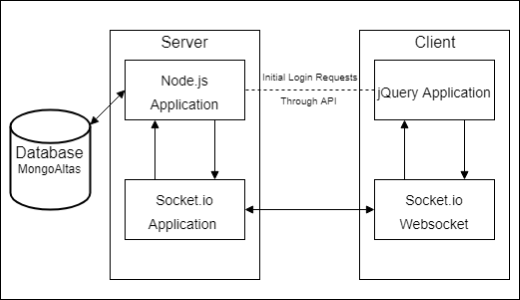
\includegraphics{arch_diagram}
	\caption{Current Design Framework of aWall Retrospective Prototype} \label{fig:archDiagram}
\end{figure}
\\
As we can see from the picture in Figure \ref{fig:archDiagram}, the participate and screen systems have direct links to server through both the sockets and through requests. The need for the socket connections to go through the server is useful for data store and manipulation before being send out, allowing for more calculation and processing strain on the server rather than the users device. 
The need for both the socket communication and requests between the server and other systems is due to the need for joining and create retrospective boards within the system. The sockets are stored within a map on the server, with needing a name that is given on joining a session to properly store the data. Therefore due to this, the need for requests is required to send data when joining a session.

The connection between the database, sockets and the server is setup during the startup of the server and remains open and available during the entire time the server is alive.

\section{Design Choices}
The technologies chosen for this project are: a jQuery frontend application, with a node.js/socket server using mongoDB as a datastore within the application. 
\begin{itemize}
	\item \textbf{jQuery:} \cite{js.foundation_2018}  This was chosen as the front-end framework for the application on the advisement of my project supervisor. This is due to the current technologies that are housed within the aWall application. jQuery was one of the technologies that was picked that is currently housed within the overall aWall prototype, allowing for simple integration between this prototype and the current aWall prototype. 
	\item \textbf{Node.js:} \cite{foundation_2018} Node.js was chosen as the backend framework due to its ability to quickly setup and integrating into other parts of the prototype through libraries such as \textit{Socket.IO} \cite{socket.io_2018} for Sockets and \textit{Mongoose} \cite{mongoose-odm-v5.1.3_2018} for MongoDB. The aWall prototype does not use Node.js as a technology, its backend framework is \textit{Python} \cite{welcome-to-python.org_2018}, this wasn't chosen due to the complexity of integration with the other technologies. 
	\item \textbf{Sockets:} \cite{socket.io_2018} Sockets were needed for this project due to the need of real-time communication within the prototype between the participant and screen systems. This was chosen due to it being one of the technologies within the current aWall prototype, therefore making it easier to integrate the two prototypes together.
	\item \textbf{MongoDB:} \cite{mongodb-for-giant-ideas_2018} MongoDB was chosen as the datastore for the prototype, this is not the datastore held within the current aWall project, as that datastore will not allow me to store the correct data needed for the retrospective section. \textit{MongoDB}, more specifically \textit{MongoAtlas} \cite{fully-managed-mongodb-hosted-on-aws-azure-and-gcp_2018} was chosen due to it's simplicity and quickness to setup and get something running. It also allows for easy integration within the backend framework with the library \textit{Mongoose} \cite{mongoose-odm-v5.1.3_2018}.
\end{itemize}
With using both jQuery and Socket.IO as the major libraries within the frontend development of the application it has will make it possible to very easily replace the backend that has been developed within this prototype and integrate this frontend into the current prototype of aWall that uses both of these technologies with next to no changes except routing points within the jQuery application.


Through the planning and start of the implementation, there has been solutions that have been looked over and removed from within the project due to not fitting within the scope required of them in the project. These are:


\begin{itemize}
	\item
\textbf{Datastore Choices:} The original aWall system used JIRA as a datastore system, connecting through their API to get the required data. JIRA was used as it was easy to integrate and get the required data for the other stages of the agile framework such as sprint planning and reviews. JIRA does not support a datastore for retrospectives, therefore it was removed as a possible solution for the datastore of the project. Due to not being able to use the datastore that was in the previous system, I have to use some form of database instead. The choice of using MongoDB was found due to its easy ability to store the required variable data that will be given from users, that I wouldn't be able to get with using a SQL database. With the use of MongoDB, I found that the use of MongoAtlas was good for the solution as it then meant I didn't need to host it locally due to that being done with Atlas. 
\end{itemize}

\section{Current Implementation Progress}
The current implementation progress within this system is as follows:
\begin{itemize}
	\item \textbf{Server:} The server has been fully setup with its socket counterpart and its connection to the datastore MongoDB. It currently has built within it a framework that allows for easy ability to add and remove extra retrospectives within itself, with 4 of the 6 retrospective types having this completed. The server is also being current hosted within the ECS system at Victoria University and can be found at: \url{http://barretts.ecs.vuw.ac.nz:52724/}
	\item \textbf{Touch:} Within the touch system, the header component with its required scope file working and also one of the retrospective methods. This header file is constant throughout the entire retrospective for the screen, it displays the most important data throughout the entire retrospective such as time elapsed, members and current stage. The work for the first retrospective type, Check-in has also been completed, with connection to the server to grab the required data for it. 
	\begin{figure}[ht]
		\centering
		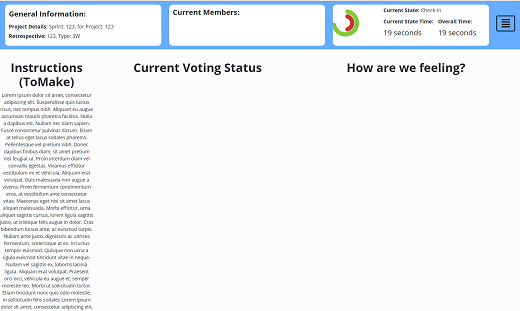
\includegraphics{moderator_progress}
		\caption{Current Progress of Screen System within aWall Retrospective Prototype} \label{fig:modProgress}
	\end{figure}

	Figure \ref{fig:modProgress} shows the current progress that has been made on the touch system as of the 3rd of June. Currently implemented within it is the header, showing all the required information such as the retrospective details, the time elapsed and the current members within the retrospective. The view that is currently shown is the only one that has been implemented, this is the check-in view for the moderator showing the three different sections that will be viewed.
	
	 \begin{figure}[ht]
	 	\centering
	 	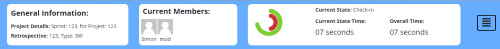
\includegraphics{header}
	 	\caption{Current Progress of Header within Screen System within aWall Retrospective Prototype} \label{fig:header}
	 \end{figure}
 
 	Figure \ref{fig:header} shows the current progress that has been made on the header as of the 3rd of June. It is split into the three sections, each containing the required information being displayed for the team of the agile retrospective. It contains the Project details such as the sprint number and project name of the retrospective, the current members connected to the board and finally the time elapsed between the current state and the overall time of the retrospective.
	
	\item \textbf{Participant:} The participant view, the only progress that has been made has been within it has been the voting system for the first retrospective and the connection to server to write the data to the datastore.
	\begin{figure}[ht]
		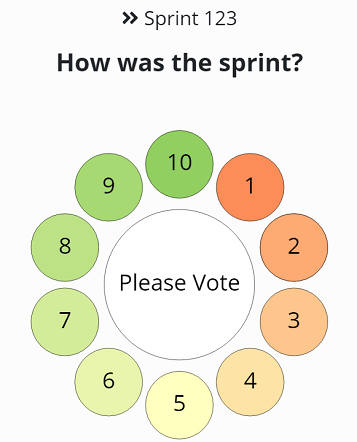
\includegraphics{participant_progress}
		\centering
		\caption{Current Progress of Participant System within aWall Retrospective Prototype} \label{fig:parProgress}
	\end{figure}


Figure \ref{fig:parProgress} shows the current progress that has been made on within the participant system with aWall. This system currently is being built with a phone in mind to interact with, but implementation will include a desktop view later on. This is the check-in view, allowing the user to vote within the retrospective.
\end{itemize}


\section{Evaluation of Solution}
The solution is going to be evaluated through User Studies. A ethics proposal has been submitted to the Human Ethics Committee within Victoria and is currently going through the process of being evaluated and approved, the ethics application number is \textit{\#0000026187}. The forms that were submitted in the application can be seen in Appendix \ref{app:ethics}. Within this user study I am looking to test on 4 -5 teams, from teams within the ENGR301/302 courses. \\
The process for the user study will consist of the following steps:
\begin{itemize}
	\item Users will volunteer and be placed into groups or 'teams' to do the retrospectives in.
	\item The teams will firstly participate within a 'control' retrospective, where they will do part of a retrospective the old way, using a cardwall.
	\item The teams will then participate in a retrospective using the aWall tool using one of the 4 main retrospective methods
	\item Finally the members within each of the teams will fill out a questionnaire about the experience of using the aWall prototype compared to the cardwall retrospective.
\end{itemize}

Using the data gathered from the questionnaires and from the observations within the user study, I will be able to not only evaluate the effectiveness of using a touch wall over a card wall, but also what retrospective method has the greatest engagement within different software teams. 

\chapter{Future Work}\label{C:future}
\section{Project Components left to complete}
\begin{enumerate}
	\item Finish development of all three components with the different retrospective types \\ \textbf{By Mid July}
	\item User study preparation \\ \textbf{By 1st August}
	\item Conduct User Study \\ \textbf{By 31st August}
	\item Analysis of User Study \\ \textbf{By 20th September}
	\item Clean up Preferred System with Software and integration within aWall prototype \\ \textbf{By 30th September}
	\item Write Final Report \\ \textbf{By 26th October}  
\end{enumerate}
\begin{figure}[ht]
	\centering
	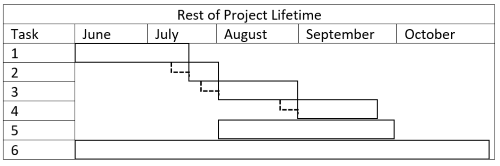
\includegraphics{timeline}
	\caption{Current timeline planned for the project}
\end{figure}


%%%%%%%%%%%%%%%%%%%%%%%%%%%%%%%%%%%%%%%%%%%%%%%%%%%%%%%

\backmatter

%%%%%%%%%%%%%%%%%%%%%%%%%%%%%%%%%%%%%%%%%%%%%%%%%%%%%%%


%\bibliographystyle{ieeetr}
\bibliographystyle{acm}
\bibliography{biblo}

\appendix
\chapter{Ethics Application Documents}
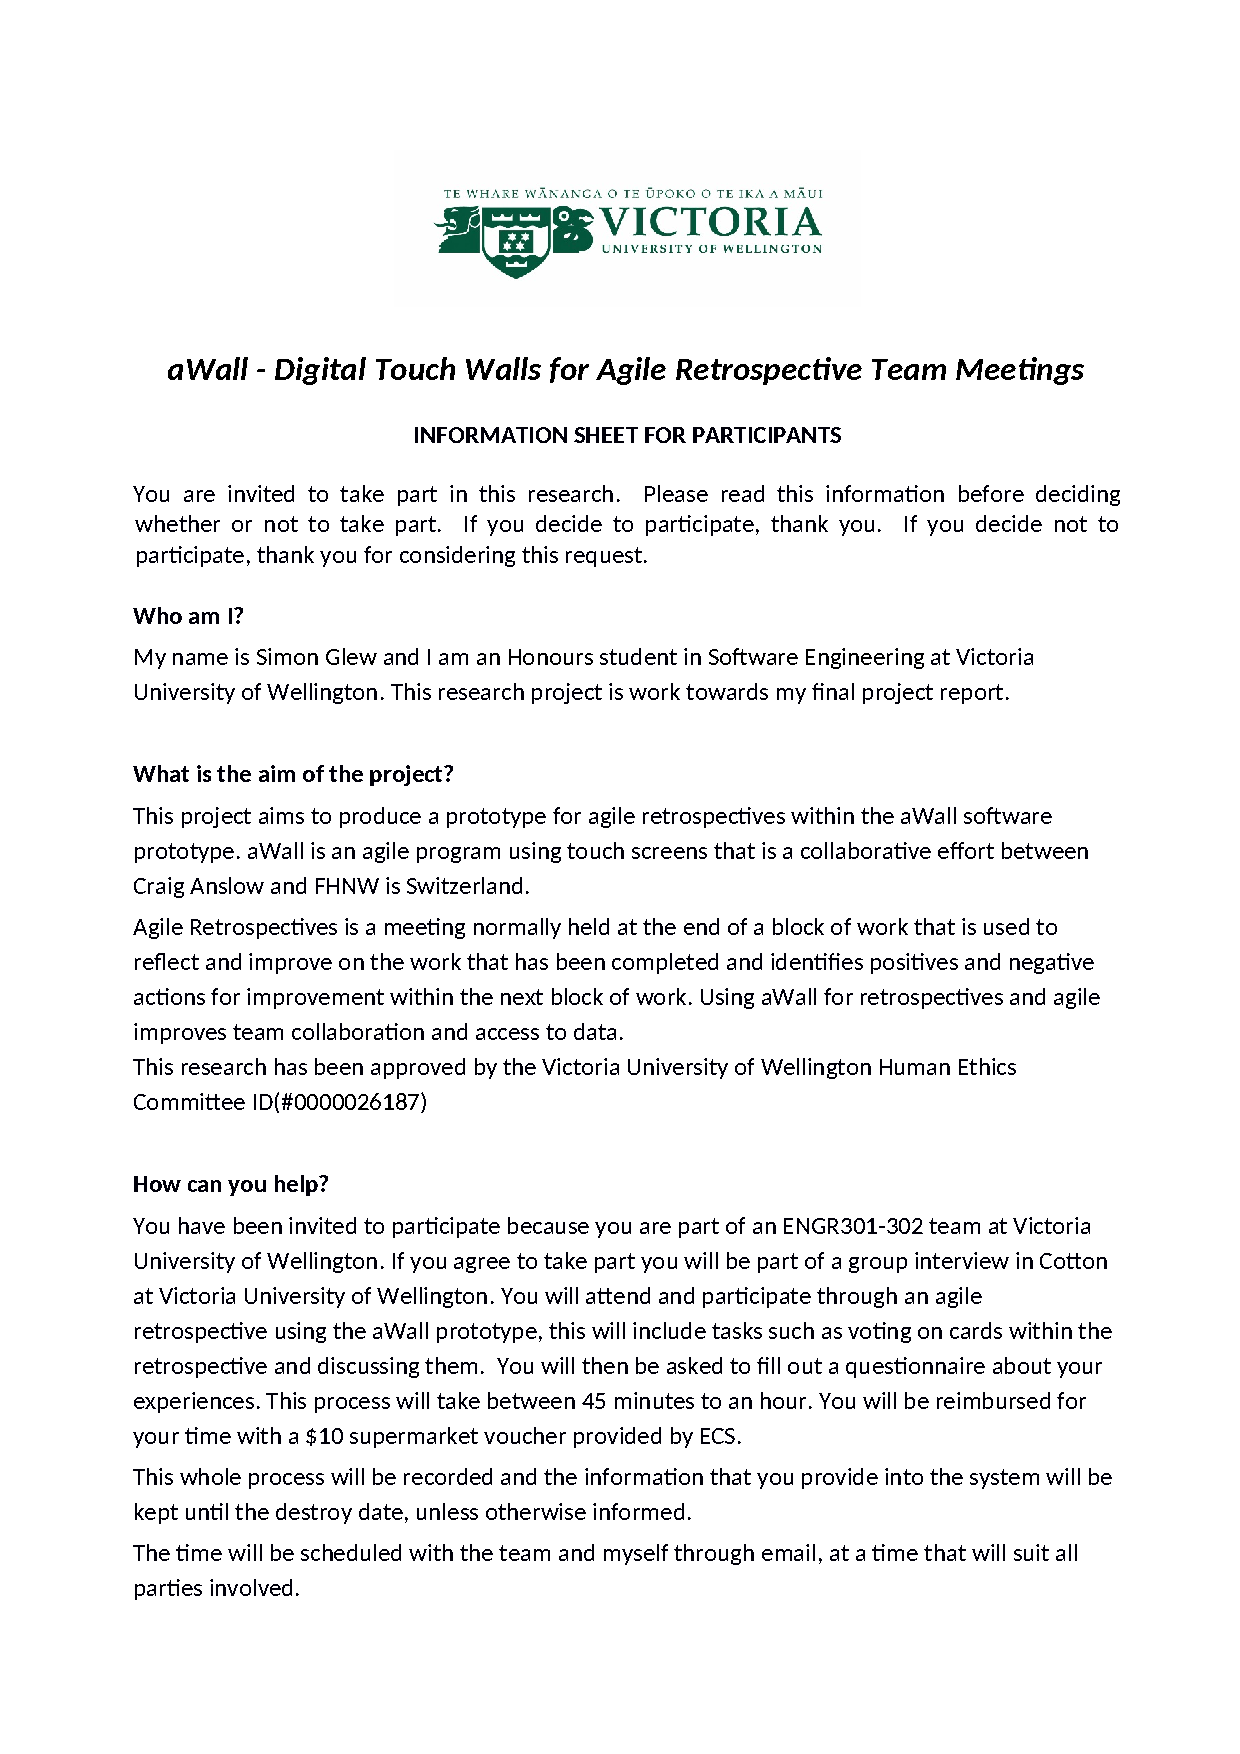
\includepdf[pages=-,scale=.95,pagecommand={\label{app:ethics}},linktodoc=true]{combined_documents.pdf}



\end{document}
